\section{Data Analysis}
    According to the data evaluation, we got $N = 204$ events. That means, we got 204 times a distance, a time and a velocity which are distributed. 
    \subsection{Data evaluation of velocity}
        We think, the velocity is a gaussian distribution. This assumption can be proven by a student's t-test. But we only have one set of data.
        \begin{longtable}{p{8cm}p{8cm}}
            \minipanf
                A\\
                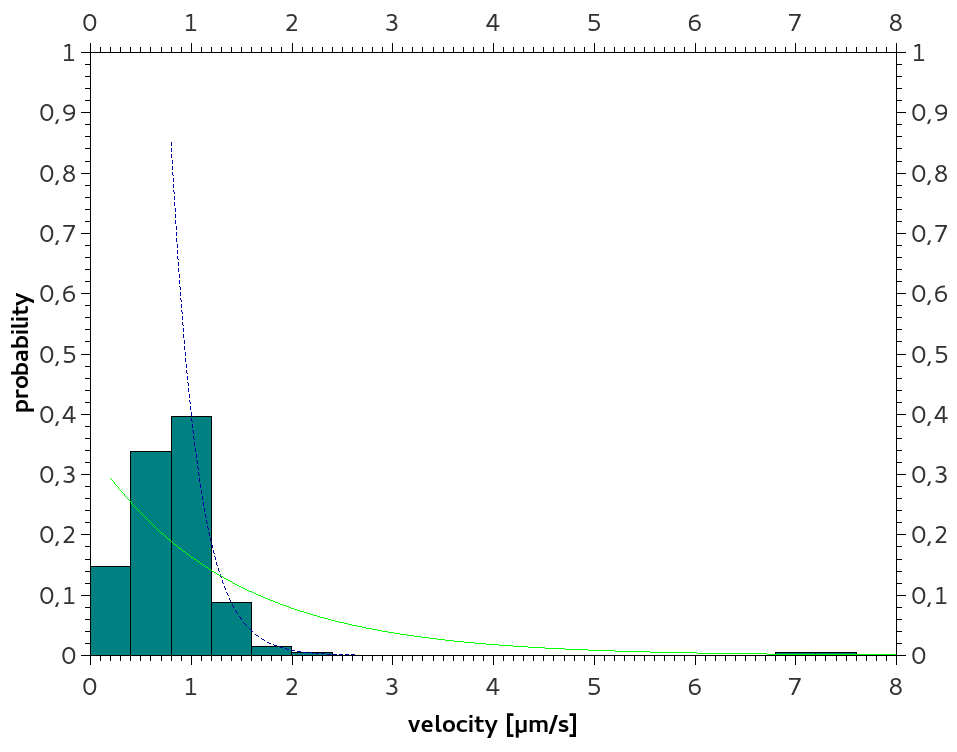
\includegraphics[scale=0.3]{pic/velodist_rel}
            \minipend
            &
            \minipanf
                B\\
                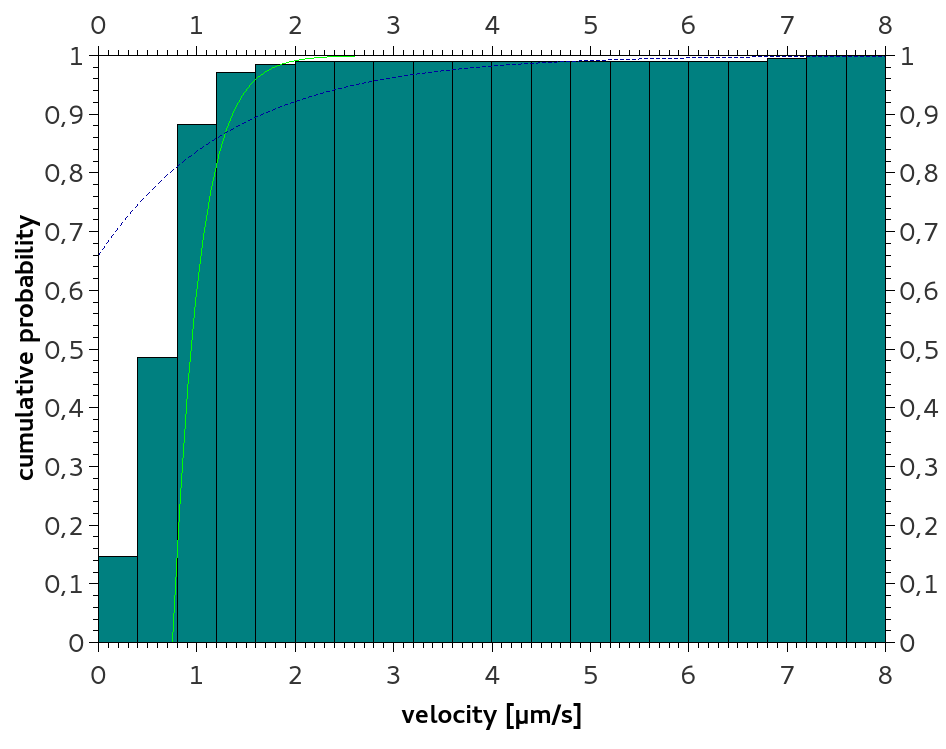
\includegraphics[scale=0.3]{pic/velocumdist}
            \minipend
        \end{longtable}
        \captionof{figure}{\textbf{A:} Histogram of the relative velocity distribution. \textbf{B:} Histogram of the cululative velocity distribution}
        \vspace{2mm}
        The mean of the velocity $\overline v$, its standard deviation $\sigma_{\overline v}$ and the standard error of the mean velocity $\Delta \overline v$ can be calculated by a data analysis tool. We used an Origin like software called qtiplot, which calculates column statistics, which are not influenced by binning, because that are the measured raw data. These include the searched values.
        In general one can calculate these values as following:
        \begin{eqnarray*}
            \overline v = N^{-1} \sum_{i = 1}^{N}v_i\ ,\ \sigma_{\overline v} = \sqrt{\sum_{i = 1}^{N} \frac{(v_i - \overline v)^2}{N}}\ , \ \Delta \overline v = \frac{\sigma_{\overline v}}{\sqrt{N}}
        \end{eqnarray*}
        So we get:
        $$ \overline v = \unit[(0.81 \pm 0.05)]{\frac{\mu m}{s}}\ , \ \ \sigma_{\overline v} = 0.72 \unit{\frac{\mu m}{s}}$$
        To minimize the error one easily take more measurements. According to the law of large numbers the measured mean velocity would vonverge to the expactation value. With an infinite number of measurements we would get the exact result. 
        Also we could use software which marks the traces, which would create a unit law of marking. As a human being, one cannot see every trace and one can not mark every trace the way. This is caused by a diameter of the traces which is not infinite. The means, one could easily stretch the distance walked by the kinesin by marking from on edge to the diagonal opposite edge. An automization would avoid these errors. 
    
    \subsection{Data evaluation of run length}